
\section{The AdEx neuron}

We choose to simulate the `AdEx' point neuron model, or the `adaptive exponential integrate-and-fire' neuron\cite{Brette2005AdaptiveExponentialIntegrateandFirea}, with conductance-based synaptic currents.
The AdEx neuron is a leaky-integrate-and-fire (LIF) neuron model, with two additions.
First, the full upstroke of each spike is simulated, as an exponential runoff.
Second, an extra dynamic variable is added: the adaptation current.
This current allows the simulation of many non-linear effects of real neurons, like spike-rate adaptation and post-inhibitory rebound.
% (Note however that we do not focus on adaptation effects in this thesis).

\marginpar{
    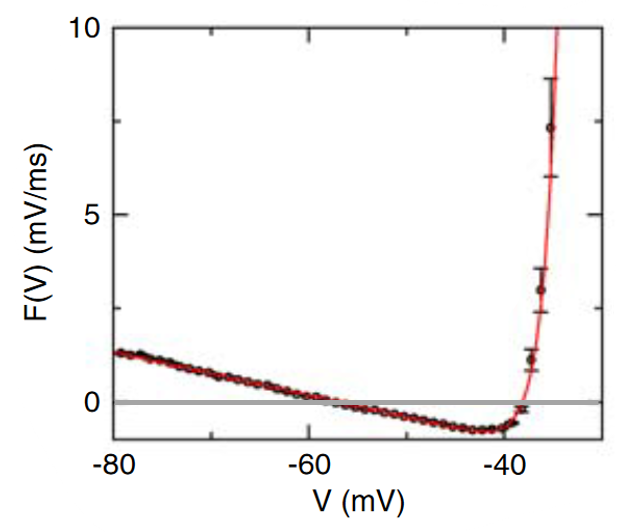
\includegraphics[w=1]{exIF-fit.png}
    \captionof{figure}{A linear-plus-exponential model (red) fit to data from a cortical pyramidal neuron (black), from \cite{Badel2008ExtractingNonlinearIntegrateandfire}}
    \label{fig:exIF-fit}
}

The AdEx model consists of two differential equations (\labelcref{eq:AdEx-V,eq:AdEx-w}), and a discontinuous update after a spike is generated (\labelcref{eq:AdEx-reset}). One equation simulates the membrane voltage $V$, and one the adaptation current $w$:
\begin{align}
    C \d{V} &=  -g_L (V - E_L)
                            + g_L Δ_T \exp \left(\frac{V-V_T}{Δ_T}  \right)
                            - I_\syn - w
                            \label{eq:AdEx-V}
                            \\[1em]
    τ_w \d{w} &= a (V - E_L) - w
        \label{eq:AdEx-w}
\end{align}

Parameters are described in \cref{tab:AdEx-params}.

The first term of \cref{eq:AdEx-V} is the restorative force pulling the voltage back to the resting (or leak) potential $E_L$. The second, exponential term is what generates the spike upstrokes. It is practically zero over most of the sub-threshold regime, and only becomes large (and then very large) near the firing threshold. (This firing threshold is characterised further on).

$I_\syn$ is the synaptic current, explained in \cref{sec:synapse_model}.
We use the sign convention of inter alia Dayan \& Abbott\footnote{\cite{Dayan2001TheoreticalNeuroscienceComputational}, ch.~5.3, p.~162} where membrane currents are defined as positive when positive charges flow \emph{out} of the cell. I.e. a positive $I_\syn$ decreases the membrane voltage (itself defined as the electric potential inside minus outside the cell).

The adaptation current $w$ decays exponentially to zero on its own ($-w$ in \cref{eq:AdEx-w}), and is influenced by voltage deviations from equilibrium: for $a > 0$, $w$ acts on $V$ in the opposite direction of the deviation, and for $a < 0$, $w$ acts in the same direction. Izhikevich calls the former a resonant current, and the latter an amplifying one.\footnote{\cite{Izhikevich2007DynamicalSystemsNeuroscience}, section 5.2.4. Note the different notation used; see the translation in \cref{tab:AdEx-Izh-compar}.}

\begin{table}[h]
    \vspace*{2em} % making space for footnote above
    \begin{sidecaption}
        {Quantities and parameters of the AdEx neuron, \cref{eq:AdEx-V,eq:AdEx-w,eq:AdEx-reset}. Values are from a model fit to a cortical regular spiking (RS) neuron, from \cite{Naud2008FiringPatternsAdaptive}. By defining the location of $\d{V}$'s minimum, $V_T$ also co-determines the location of the firing threshold.}
        [tab:AdEx-params]
        \begin{tabular}{c l r}
            Name  & Description & Value \\
            \hline
            $V$  & Membrane voltage & (in mV) \\
            $w$   & Adaptation current & (in pA) \\
            $C$ & Membrane capacitance & $104$ pF \\
            $g_L$ & Input / leak conductance & $4.3$ nS \\
            $E_L$  & Resting / leak potential & $-65$ mV \\
            $Δ_T$  & Threshold slope factor & $0.8$ mV \\
            $V_T$  & Location of minimum of $\d{V}$ & $-52$ mV \\
            $τ_w$   & Time constant of adaptation current & $88$ ms \\
            $a$ & Sensitivity of adaptation current to $V$ & $-0.8$ nS \\
            $θ$ & Spike definition threshold & $40$ mV \\
            $V_r$  & Reset voltage after spike & $-53$ mV \\
            $b$ & Adaptation current bump after spike & $65$ pA
        \end{tabular}
    \end{sidecaption}
    \vspace*{1em}
\end{table}

In this chapter, we will analyse $\d{V}$ as a function of $V$, i.e. analyse it as a dynamical system: will the voltage increase or decrease at the current voltage?
For conciseness, we call this function $F(V)$. I.e. $F(V) = \d{V} =$ the right-hand-side of \cref{eq:AdEx-V} here, scaled by $1/ C$. We'll mostly analyse $F$ in the absence of synaptic and adaptation currents, i.e. for $I_\syn$ and $w$ both zero.
\Cref{fig:exIF-fit} shows the $F(V)$ curve for an AdEx neuron fit to a real neuron. \Cref{fig:Vm_Izh_vs_AdEx} compares the $F(V)$ curve of an AdEx neuron  with that of another two-dimensional neuron model, the Izhikevich neuron.

In addition to the two differential equations, the AdEx model also consists of an instantaneous reset condition. When the membrane voltage $V$ reaches a certain threshold $θ$, a spike is recorded, $V$ is reset, and $w$ is increased:
\begin{align}
    \text{if}\ V > θ\ \text{then:}\ \label{eq:AdEx-reset}
    & V ← V_r \\
    & w ← w + b \notag
\end{align}
This bump of the adaptation current is what provides the spike rate adaptation: the more spikes the neuron has recently fired, the higher the adaptation current $w$ and the more it drives down the voltage (\cref{eq:AdEx-V}), away from the firing threshold.

For a full description of the different firing patterns that the AdEx neuron can exhibit, for different parameter values (i.e, a characterisation of its bifurcations), see \cite{Naud2008FiringPatternsAdaptive}, \citetitle*{Naud2008FiringPatternsAdaptive}.
For an even fuller description, including a derivation of two-dimensional neuron models from higher-dimensional, Hodgkin-Huxley-like models, see Eugene Izhikevich's book, \citetitle*{Izhikevich2007DynamicalSystemsNeuroscience} \cite{Izhikevich2007DynamicalSystemsNeuroscience}.

In terms of parameter choice, we choose to simulate a cortical regular spiking (RS) neuron, i.e. a `standard' excitatory neuron that does not display e.g. bursting or fast-spiking behaviour. We take our parameter values from \cite{Naud2008FiringPatternsAdaptive}\footnote{Section 6, and Table 1, row 3}, where they fitted an AdEx model to recordings from real cortical RS neurons injected with different step currents. Parameter values are listed in \cref{tab:AdEx-params}.

Examples of the signals $V$ and $w$ that this model generates are given later, in \cref{fig:impulse_response} and \cref{fig:all_sigs_6500}.

% Slowly injecting current $I$ shifts Izhikevich's parabola upwards, raising the resting potential and lowering the spiking threshold. At a certain point, the two fixed points merge and disappear ("annihilate"), in a "saddle--node"\fnm or "fold" bifurcation. The voltage can only go up -- and with the reset of \cref{eq:Izh_V_reset}, the neuron keeps spiking.

% \fnt{In the full $(V, u)$ phase plane, at $V_r$ there is a node (both eigendirections are attracting), and at $V_t$ there is a saddle (only one eigendirection attracts, the other repels). Hence, "saddle--node" bifurcation.}

% On the other hand, negative input currents or a positive adaptation current $u$ shift $\dot{V}$ downwards, giving a lower resting potential and a higher spiking threshold. This is how the model creates spike rate adaptation: every spike increases $u$ (\cref{eq:Izh_u_update}), and thus the spiking threshold.


\subsection{Analysis}

Where are the fixed points of the dynamical system $\d{V} = F(V)$? I.e, where is $F = 0$? Like other neuron models, there are two fixed points: a stable one at the leak potential $E_L$, and an unstable one at the instantaneous firing threshold (which we'll call $E_T$).

We see in \cref{eq:AdEx-V} (for $I_\syn = 0$ and $w = 0$) that the leak potential $E_L$ is indeed a fixed point -- or rather lies very close to one: the exponential term is negligibly small at $V = E_L$.
\marginpar{
    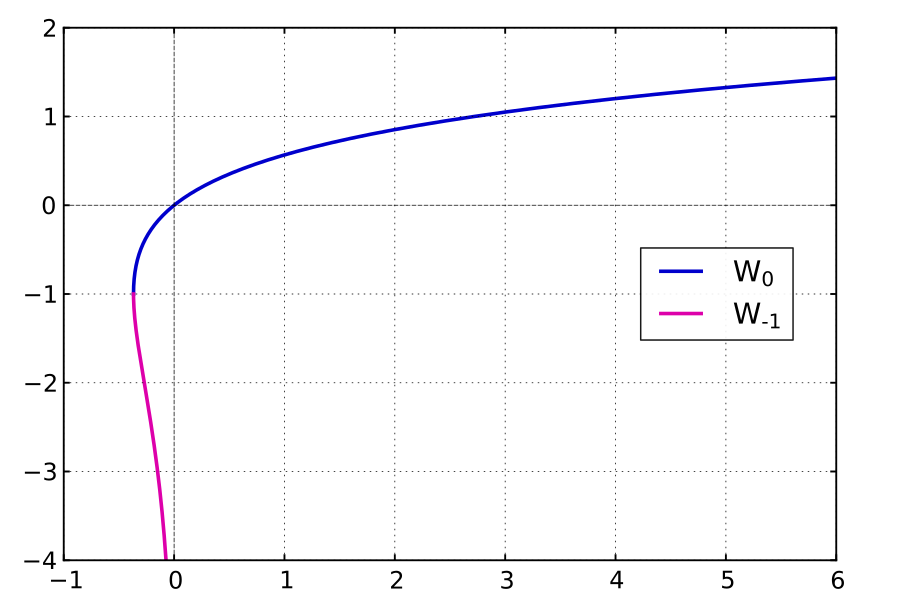
\includegraphics[w=1]{LambertW.png}
    \captionof{figure}{The Lambert $W$ functions for real numbers.}
    \label{fig:LambertW}
}
The second fixed point has no straightforward expression. The exact solutions for $F$'s roots need the so called Lambert $W$ or `product logarithm' functions $W_0$ and $W_{-1}$ (see \cref{fig:LambertW}). The roots are found at:
\begin{equation}
    V = E_L - Δ_T W_k \left( -\exp\left( \frac{E_L - V_T}{Δ_T} \right) \right) \label{eq:LambertW}
\end{equation}
..where $k = 0$ gives the resting potential, and $k = -1$ the instantaneous firing threshold.\footnote{
    Here too we see that the true resting potential is almost identical to $E_L$: $W_0$ passes through zero, and its argument is $≈ 0$, because the exponential's argument is negative. For $W_{-1}$ however, \cref{fig:LambertW} shows that the second term is not negligible around $0$.}
For our cortical RS neuron, this gives us an instantaneous threshold of $E_T = -49.6$ mV.

% source:
% - https://www.wolframalpha.com/input?i=real+roots+of+f%28V%29+%3D+-g*%28V-L%29%2Bg*D*exp%28%28V-T%29%2FD%29
% - https://www.wolframalpha.com/input?i=L+-+D+ProductLog%28-1%2C+-e%5E%28%28L+-+T%29%2FD%29%29+for+L%3D-65%2C+D%3D0.8%2C+T%3D-52

Also of interest -- especially when comparing with the Izhikevich neuron later -- is the slope of AdEx's $F(V)$, i.e. its derivative with respect to $V$:
\begin{align}
    \d[V]{F} &= \dd{V} \left( -g_L (V - E_L)
         + g_L Δ_T \exp\left(\frac{V - V_T}{Δ_T}\right) \right) \notag \\
    &= -g_L + g_L \exp\left(\frac{V - V_T}{Δ_T}\right) \label{eq:dFdV}
\end{align}
This derivative is zero at $V = V_T$. I.e, unlike what is suggested by the `$T$' subscript, and the name `effective threshold potential' given to it in the AdEx literature\cite{Brette2005AdaptiveExponentialIntegrateandFirea,Naud2008FiringPatternsAdaptive}, $V_T$ is not the instantaneous threshold potential (it is not a zero of $F$), but rather the minimum of $F$ (it is the zero of $\d[V]{F}$).

From \cref{eq:dFdV}, we also calculate the slope of $F$ at its two roots. At $V = E_L$, the slope (also known as the leak or input conductance here) is $-g_L$, plus a negligibly small exponential term. The negative sign shows that this is a stable fixed point: in a linearization of $F$ around this point, at voltages below the resting potential, $F$ (i.e. $\d{V}$) is positive and thus $V$ will increase. At voltages above $E_L$, $F$ is negative and $V$ will decrease. Small deviations on either side of the resting potential will thus decay back to this resting potential.

At the firing threshold $V = E_T$ (i.e. the second solution to \cref{eq:LambertW}), the slope is:
\begin{equation}
    g_L \left( \exp\left(\frac{E_T - V_T}{Δ_T}\right) - 1 \right)  \label{eq:AdEx-slope}
\end{equation}
..which is positive (as $E_T > V_T$), indicating that this is an unstable fixed point: a small deviation of the voltage above $E_T$ will blow up to infinity (i.e, a spike is generated).


\section{Alternative neuron models}

Why did we choose the AdEx model to simulate neuron voltages? In short, because it strikes a good balance between realism and complexity. We briefly consider here two alternative neuron models: the simple leaky-integrate-and-fire (LIF) neuron, and the more complex Hodgkin-Huxley (HH) neuron.
In the next section, we go into more depth on a third alternative, the very similar Izhikevich neuron.

A simpler model than AdEx would be the well-known LIF neuron:
\begin{align*}
    C \d{V} =  -g_L (V - E_L) - I_\syn \\[1em]
    \text{if}\ V > θ,\ \text{then:}\ V ← V_r \\
\end{align*}
As is apparent from comparing this with \cref{eq:AdEx-V,eq:AdEx-reset}, the AdEx model is an extension of the LIF model. The LIF neuron lacks a simulation of the upstroke of spikes (the exponential term in \cref{eq:AdEx-V}), and the slower time-scale adaptation current (\cref{eq:AdEx-w}), which allows the simulation of many qualitatively different real neuron types.
It is especially this first addition, the full upstroke simulation, that seems relevant in generating realistic voltage traces.

Would this thesis have been very different had we used LIF neurons instead?
Probably not, though it might depend on the mean voltage level of the simulated neuron: if it is well below the firing threshold, both LIF and AdEx are linear (the exponential term is negligible), and they behave quasi identically. When a spike is generated in the AdEx model, the exponential feedback makes the upstroke very fast, and thus not many timesteps in the simulation are spent on it, versus the linear regime.

On the other hand, when the neuron would continuously teeter just below its firing threshold, the LIF and AdEx models do not behave similarly. LIF's $F(V)$ curve is still fully linear, while AdEx's is not, and AdEx will behave more like a real neuron -- see \cref{fig:exIF-fit}.

Another well-known alternative neuron model is the class of Hodgin-Huxley (HH)-like neurons. These models simulate the full trajectory of a spike: both its upstroke and its downstroke. Unfortunately they also have many free parameters. They also take a bit longer to simulate, being higher dimensional (having more differential equations), and containing many more exponential terms, which take the brunt of the time when numerically evaluating a differential expression.



\clearpage
\section{The Izhikevich neuron}

\begin{figure}
    \begin{sidecaption}
        {Neuron models as dynamical systems: a comparison of the $F(V)$ curves of the Izhikevich and AdEx neurons. `Experimental' is an AdEx neuron fit to a cortical pyramidal neuron (using data from \cite{Badel2008ExtractingNonlinearIntegrateandfire}). The Izhikevich neuron's parameters were chosen to match the fixed points and the leak conductance. Arrows indicate whether the voltage will increase or decrease (1D flow field). →~\textbullet{}~← is a stable fixed point (resting potential), ←~o~→ is an unstable fixed point (spike threshold). $\dot{V} ≡ \d{V}$.}
        [fig:dynsys]
        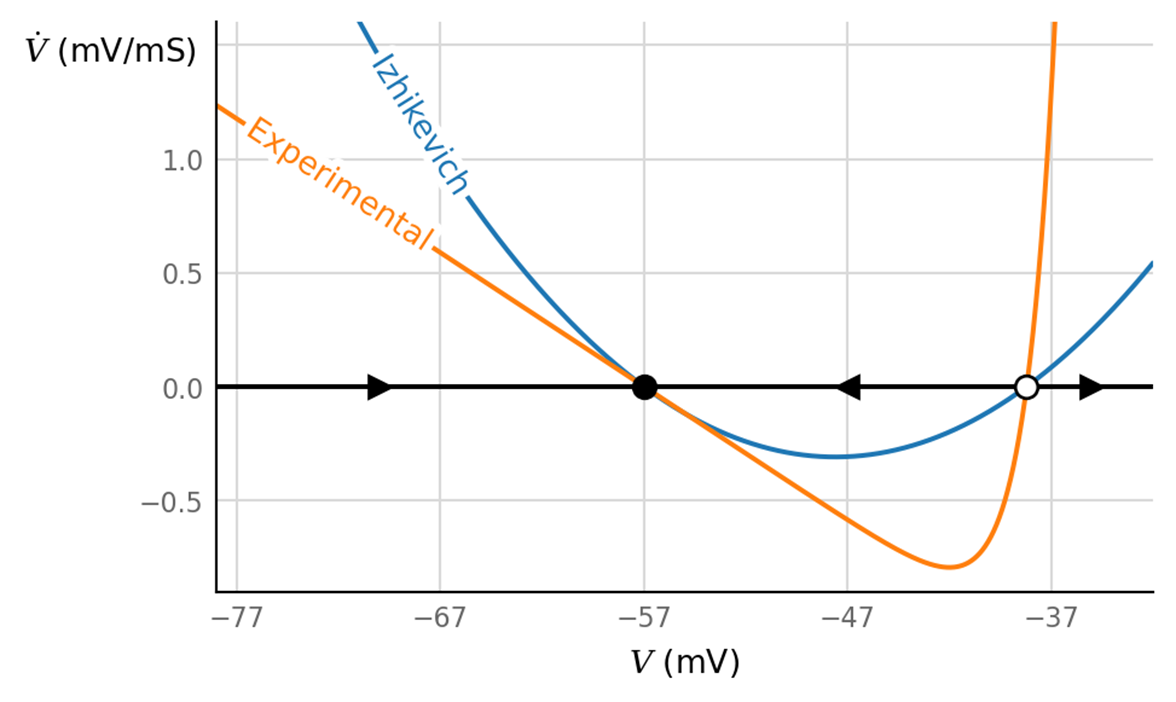
\includegraphics[w=0.9]{dynsys.png}
    \end{sidecaption}
\end{figure}

Another alternative neuron model is the Izhikevich neuron, which is exceedingly similar to the AdEx neuron.
These are the Izhikevich equations, using the same symbols as used before (in \cref{eq:AdEx-V,eq:AdEx-w,eq:AdEx-reset}):
\begin{align}
    C \d{V} &=  k (V - E_L) (V - E_T) - I_\syn - w  \label{eq:Izh-V}  \\[1em]
    τ_w \d{w} &= a (V - E_L) - w     \label{eq:Izh-w} \\[2em]
    \text{if}\ V& > θ,\ \text{then:}  \label{eq:Izh-reset} \\
        &V ← V_r \notag \\
        &w ← w + Δw \notag
\end{align}

We have introduced two new parameters not present in the AdEx equations: the steepness of the parabola, $k$; and $E_T$, the instantaneous firing threshold (the firing threshold in the absence of any synaptic or adaptation currents).

The only difference with AdEx is in \cref{eq:Izh-V}, where the $F(V)$ curve is not made by a linear plus exponential term, as in AdEx; but rather by a quadratic (a parabola). Its two zeros (the fixed points) are readily apparent, as $E_L$ and $E_T$.


\subsection{Correspondences with AdEx}

In Izhikevich's book\footnote{\cite{Izhikevich2007DynamicalSystemsNeuroscience}, section 5.2.4, equations 5.7 \& 5.8}, different names are used for the same quantities:
\begin{align}
    C \d{v} &= k(v - v_r)(v-v_t) - u + I \label{eq:IzhIzh-v} \\[1em]
    \d{u} &= a(b(v-v_r) - u) \\[2em]
    \text{if}&\ v > v_\text{peak},\ \text{then:} \\
    v &← c  \notag \\
    u &← u + d  \notag
\end{align}

\Cref{tab:AdEx-Izh-compar} compares both notation conventions.

\begin{table}[h]
    \begin{sidecaption}
        {Different symbols used for the same quantities, in \cite{Brette2005AdaptiveExponentialIntegrateandFirea} and in most of this thesis (`AdEx') , and in \cite{Izhikevich2007DynamicalSystemsNeuroscience} (`Izh').
        Membrane capacitance $C$ (in farad) is the same in both notations.}
        [tab:AdEx-Izh-compar]
        \begin{tabular}{c c l c}
            AdEx   & Izh  & Description & Units \\
            \hline
            $V$  & $v$   & Membrane voltage & V \\
            $w$  & $u$   & Adaptation current & A \\
            $τ_w$  & $1/a$   & Time constant of adaptation current & s \\
            $E_L$  & $v_r$  & Resting / leak potential & V \\
            $V_r$  & $c$  & Reset voltage after spike & V \\
            $a$  & $b$ & Sensitivity of adapt. current to $V$ & S \\
            $b$  & $d$ & Adaptation current bump after spike & A \\
        \end{tabular}
    \end{sidecaption}
\end{table}

Beside these straightforward correspondences, there are some parameters in either model that have no direct equivalent in the other: $k$ and $v_t$ in Izhikevich, and $g_L$, $Δ_T$, and $V_T$ in AdEx.
For those, we'll look at the shape of Izhikevich's $F(V)$, as we've done for the AdEx neuron before.

First, the AdEx parameter $g_L$. This is the input conductance, a.k.a. the leak conductance, and the slope of $F(V)$ around the leak potential. We can find this same conductance for the Izhikevich neuron by taking the derivative with respect to $v$ of the right hand side of \cref{eq:IzhIzh-v}, at $w = 0$, $I_\syn = 0$, and $v = v_r$. We find:
\begin{equation}
    \dd{v}(k(v-v_r)(v-v_t)) \Big|_{v=v_r} = k(v_r - v_t)
\end{equation}
(this value is negative: the leak potential is a stable fixed point. This corresponds to \cref{eq:AdEx-V}, where we find `$-g_L$').
Thus, our first nontrivial correspondence:
\begin{equation}
    g_L = k (v_t - v_r)  \label{eq:leak_conductance}
\end{equation}

We've seen that $V_T$ is the minimum of AdEx's $F$.
The minimum of Izhikevich's $F$ is easily found as the average of the parabola's two zeros. I.e, $V_T$ corresponds to $(v_r + v_t) / 2$.

Finally, $Δ_T$ co-determines the slope of AdEx's $F$ at the firing threshold (\cref{eq:AdEx-slope}). Given that Izhikevich's $F$ is a parabola, with slopes equal in magnitude at both roots, we already know the firing threshold slope: it is the same as the leak conductance, \cref{eq:leak_conductance}.\\
Here, the AdEx model is more expressive than Izhikevich's: the slope of $\d{V}$ at the firing threshold can be independently tweaked from the leak conductance; in Izhikevich these two are clung together by the form of the quadratic equation.

\FloatBarrier
\subsection{Comparison with AdEx}

The Izhikevich and AdEx models are very similar. Their phase spaces are topologically identical:
the adaptive current equation is identical (up to a renaming of the variables); and the $F(V)$-graph has the same shape, with two fixed points: a stable fixed point at the resting potential, and an unstable one at the firing threshold (\cref{fig:dynsys}).

They differ in the exact shape: Izhikevich's $F(V)$ is a parabola, while AdEx is the more realistic `linear subthreshold, and then transitioning to an exponential' (see \cref{fig:exIF-fit,fig:dynsys}).
As a result, Izhikevich neurons have an unrealistically slow spike upstroke, examples of which can be seen in \cref{fig:Vm_Izh_vs_AdEx}.

\begin{figure}
    \hspace*{10em}
    \includegraphics*[w=1.4]{Vm_Izh_vs_AdEx.pdf}
    \captionn{Two neuron models behave differently for (near) identical parameters and input}{
    \small{The AdEx neuron's parameters are from \cite{Naud2008FiringPatternsAdaptive}, for a cortical regular spiking neuron. The Izhikevich neuron's parameters are copied from the AdEx neuron wherever they correspond directly. The other parameters are chosen so both models have the same resting and threshold potentials, and the same leak conductance, using the correspondences found earlier in this section. Both models receive EI-balanced synaptic input from 6500 Poisson spike trains with lognormal firing rates. The AdEx neuron was given stronger inputs ($Δg_\exc = 12.2$ pS) than the Izhikevich neuron ($Δg_\exc = 4$ pS), so as to obtain the same number of output spikes. (In both cases, $Δg_\inh = 4\ Δg_\exc$). For more details, see \nburl{2023-06-23__Vm_traces_AdEx_Izh__Brian}.}}
    \label{fig:Vm_Izh_vs_AdEx}
\end{figure}

\begin{figure}
    \hspace*{10em}
    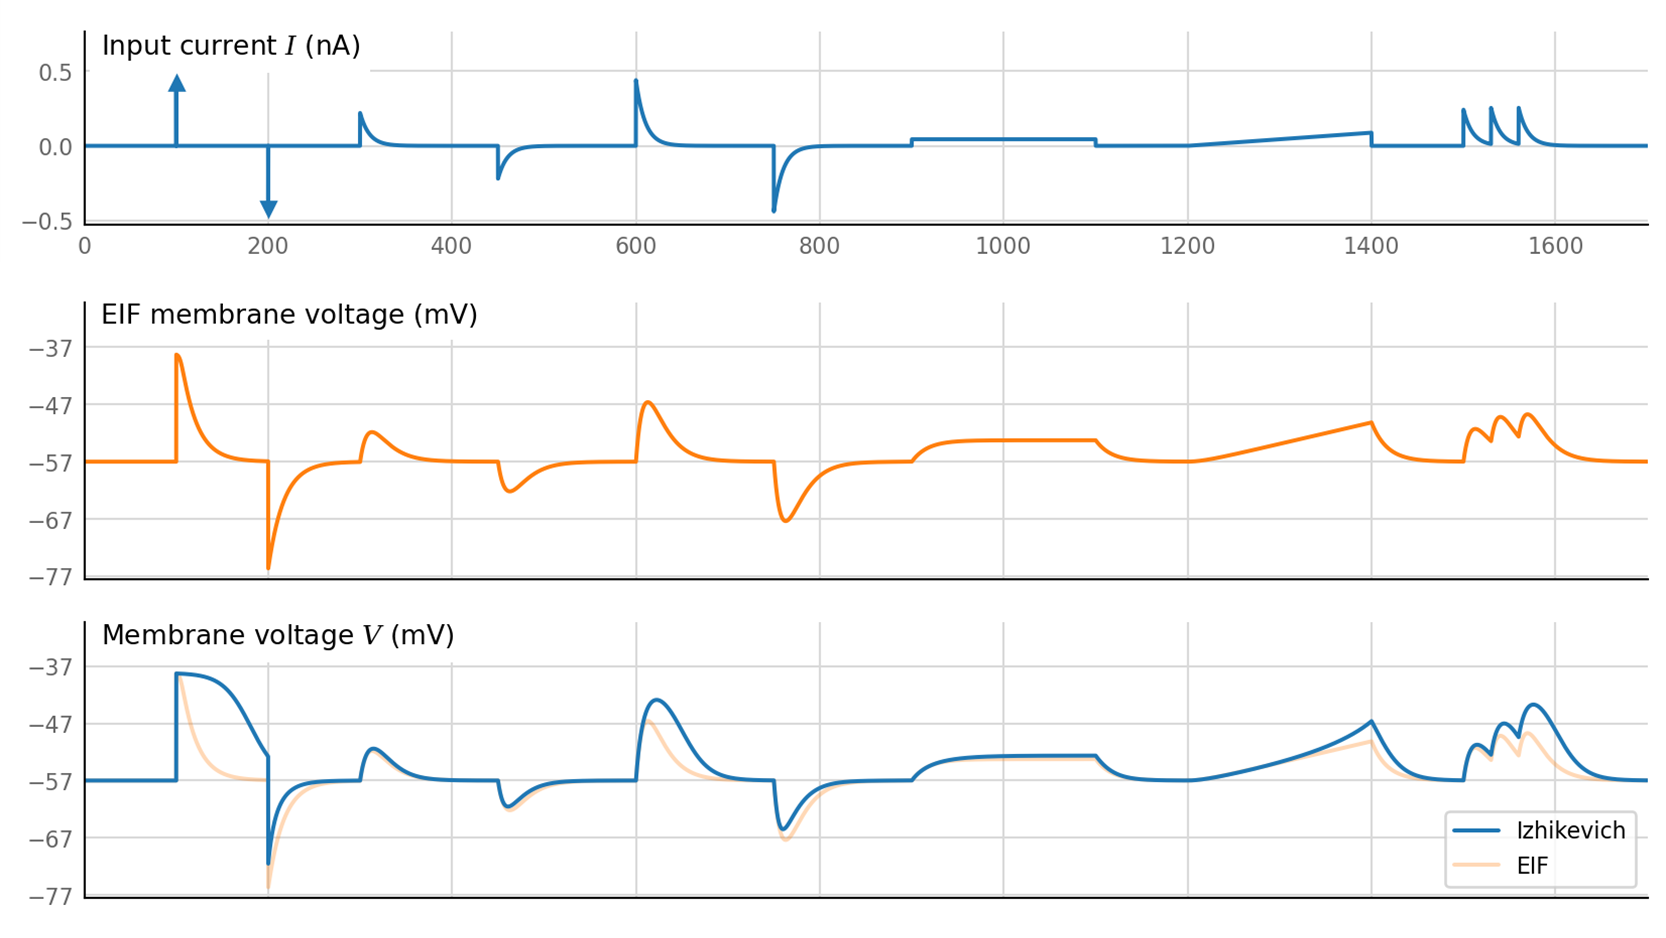
\includegraphics[w=1.5]{testbench-I-Izh-EIF.png}
    \captionn{The nonlinear response of Izhikevich neurons to subthreshold input currents}{`EIF' stands for exponential integrate-and-fire; it has the same $\d{V}$ as an AdEx neuron. Adaptation currents are negligibly small for both models in this test scenario.
    % Izhikevich parameters from \cite{Izhikevich2007DynamicalSystemsNeuroscience,Humphries2006UnderstandingUsingIzhikevich}, for a Cortical Regular Spiking neuron.
    % EIF parameters chosen to match: $C = 100$ pF, $E_L = -60$~mV, $R = 80\, \si{\mega\ohm}$.
    }
    \label{fig:testbench-I-Izh-EIF}
\end{figure}

A second issue is Izhikevich's subthreshold nonlinearity. The effects of this can be seen in \cref{fig:testbench-I-Izh-EIF}. Positive input currents produce stronger responses than equally large negative input currents. This is explained by the quadratic $\d{V}$ shape: positive deviations are attenuated less, and negative deviations more, than a linear neuron would. Real and AdEx neurons do not suffer this assymetry.

This nonlinearity is not visible for small voltage deviations, which is what the postsynaptic potentials we are interested in in this thesis tend to be. There is however an effect of the neuron's average voltage: if this voltage is constantly on the higher side, then inputs -- both negative and positive -- will cause larger responses than if the median voltage was lower.


\clearpage
\section{Synapse model}
\label{sec:synapse_model}

One as of yet unexplained term in our neuron model, \cref{eq:AdEx-V}, is the synaptic current $I_\syn$.
This is the following sum over all input synapses $i$ of the neuron:
\begin{equation}
    I_\syn = \sum_i g_i (V - E_i)
    \label{eq:I_syn}
\end{equation}
where $V$ is the global membrane voltage of the neuron, $E_i$ is the reversal potential of that synapse, and $g_i$ is the local synaptic conductance, which is modulated by presynaptic spikes.

For an excitatory synapse, $V < E_i$, making $g_i (V - E_i)$ negative, increasing the membrane voltage according to the sign convention for $I_\syn$ in \cref{eq:AdEx-V}.

We simulate the synaptic conductances $g_i$ as exponentially decaying signals (with time constant $τ_g$), and bump them up instantaneously on arrival of a presynaptic spike:
\begin{gather}
    \d{g_i} = -g_i / τ_g
    \label{eq:g_i}
    \\[1em]
    \text{On incoming presynaptic spike:}\notag\\
    \ g_i ← g_i + Δg_i
\end{gather}

\marginpar{
    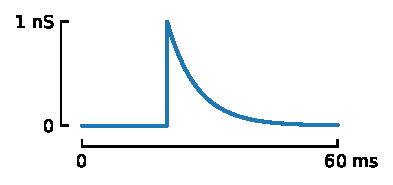
\includegraphics{g1.pdf}
    \captionof{figure}{Example synaptic conductance trace $g_1(t)$, with a single incoming spike at $t = 20$~ms.}
    \label{fig:g1}
}
\marginpar{
    \vspace*{3em}
    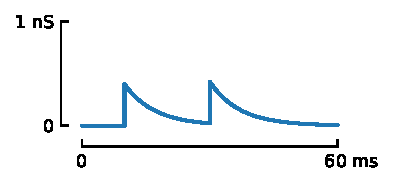
\includegraphics{g2.pdf}
    \captionof{figure}{Another example trace $g_2(t)$, with spikes at $t = 10$~ms and $30$~ms, and a smaller $Δg$.}
    \label{fig:g2}
}

Note that these are not the so called alpha-synapses. Those are two dimensional and also have an exponential rise, instead of just an exponential decay. (For an infinitely fast rise though, these models are of course the same).
Simulating a full alpha synapse might increase the realism of our voltage traces, for a small simulation cost. We did not try this however. Foremost because alpha synapses fit to real data often have very fast rise times that are almost indistinguishable from instantaneous jumps.

For efficiency, we give all our excitatory synapses the same reversal potential, $E_\exc$. Idem for the inhibitory synapses, with $E_\inh$. This allows us to factor the synaptic current sum (\cref{eq:I_syn}) as follows:
\begin{equation}
    I_\syn = (V - E_\exc) \sum_{\exc\ i} g_i \  + \  (V - E_\inh) \sum_{\inh\ i} g_i
    \label{eq:I_syn_factor}
\end{equation}

The sums of conductance signals $g_i(t)$ can also be simplified. Say that the values of $g_i$ at $t = 0$ are $G_i$. The solution to \cref{eq:g_i} (at least in the time until a new presynaptic spike arrives) is then
\begin{equation}
    g_i(t) = G_i\ e^{-t/τ_g}
\end{equation}

With this, and when all synapses have the same time constant $τ_g$, the two sums in \cref{eq:I_syn_factor} can be factored as follows:\footnotemark
\footnotetext{
    This is only valid in the time before any new spikes arrive.
    But the `summability' still holds after a new spike.
    To see this, the given reasoning can be repeated, but simply with different values for the $G_i$ (all decayed by an amount $e^{-t_\text{spike}/τ_g}$, and one increased by a bump $Δg_i$), and then redefining $t_\text{spike}$ to be $t = 0$.
}
\begin{equation}
    \sum_i g_i(t) = \sum_i \left( G_i\ e^{-t/τ_g} \right)
                            = \left( \sum_i G_i  \right) e^{-t/τ_g}
\end{equation}
This means that we need to only keep track of two conductance signals: $g_\exc$ and $g_\inh$, each the sum of all excitatory or all inhibitory synaptic conductances.

\marginpar{
    \vspace*{2em}
    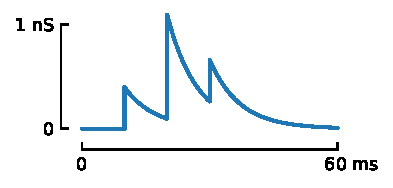
\includegraphics{g3.pdf}
    \captionof{figure}{A third synaptic conductance trace $g_3(t)$, with three input spikes at the same times and strengths as in \cref{fig:g1,fig:g2}. This signal is simulated independently, but turns out to be equal to the sum of the two others: $g_3(t) ≡ g_1(t) + g_2(t)$.}
}

Our synaptic current sum then becomes simply:
\begin{equation}
    I_\syn = (V - E_\exc)\ g_\exc \  + \  (V - E_\inh)\ g_\inh,  \label{eq:I_syn_simple}
\end{equation}
and we only need to simulate two differential equations, instead of one for every synapse:
\begin{align}
    \d{g_\exc} &= -g_\exc / τ_g  \label{eq:dge-dgi} \\
    \d{g_\inh} &= -g_\inh / τ_g, \notag
\end{align}
where on arrival of a spike at synapse $i$ either $g_\exc$ or $g_\inh$ is instantaneously increased by a value $Δg_i$, depending on whether that synapse is excitatory or inhibitory.

We choose an excitatory reversal potential of $E_\exc = 0$~mV, an inhibitory one of $E_\inh = -80$~mV, and a time constant for the synaptic conductance decay of $τ_g = 7$~ms. These values are rather arbitrary, but in line with other simulation studies (e.g. \cite{Brette2007SimulationNetworksSpiking}).


\section{Model summary}
\label{sec:model-summary}

Combining \cref{eq:AdEx-V,eq:AdEx-w,eq:AdEx-reset} with \cref{eq:I_syn_simple,eq:dge-dgi}, our complete AdEx point neuron with conductance-based synaptic current is:

\begin{align*}
    & C \d{V} =  -g_L (V - E_L)
                            + g_L Δ_T \exp \left(\frac{V-V_T}{Δ_T}  \right) \\
                            & \hspace*{4em}
                            \underbrace{- g_\exc (V - E_\exc)  - g_\inh (V - E_\inh)}_{-I_\syn}
                            \ - \ w \\[1em]
    & τ_w \d{w} = a (V - E_L) - w \\[1em]
    & τ_g \d{g_\exc} = -g_\exc  \\[1em]
    & τ_g \d{g_\inh} = -g_\inh
\end{align*}
\marginpar{
    % \vspace*{-1em}
    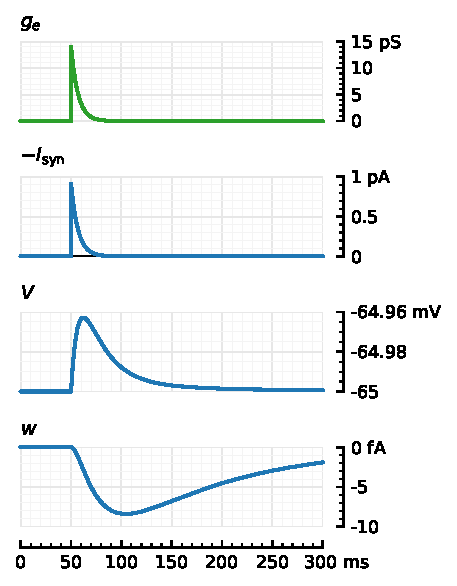
\includegraphics[w=1.07]{impulse_response}
    \captionof{figure}{
        \textbf{Impulse response of the conductance-based AdEx neuron},
        \small{using a single excitatory input spike arriving at $t = 10$~ms, with a synaptic weight $Δg_\exc$ of 14 pS. Parameters as in \cref{tab:AdEx-params}, with $E_\exc = 0$~mV and $τ_g = 7$~ms. More details at \nburl{2023-07-26__AdEx_Nto1_we_I_syn}.}}
    \label{fig:impulse_response}
}
\begin{alignat*}{2}
    & \text{When}\ V > θ \text{:}  &&   V \ ← \ V_r \\
    & && w \ ← \ w + b \\[1em]
    & \text{On input spike at..} \\
    & \qquad \text{exc. synapse } i \text{:} \hspace*{3em}
        && \ g_\exc \ ← \ g_\exc + Δg_i \\
    & \qquad \text{inh. synapse } j \text{:}  \hspace*{3em}
        && \ g_\inh \ ← \ g_\inh + Δg_j
\end{alignat*}

We solve these equations numerically using first-order (Euler) integration, with a timestep $Δt$ of $0.1$ ms. This timestep is sufficiently small with respect to the different time constants in the model\footnote{$τ_g = $~7~ms,\\$τ_w = $~88~ms,\\$C / g_L = $~24.2~ms.}. See \cref{sec:software} below for more details on the numeric implementation.

\Cref{fig:impulse_response} shows the impulse response of this model, using a single incoming excitatory spike. The PSP bump is visible in the third panel. Note its tiny size, of about 0.04~mV. Our task will be to detect this tiny signal, in a sea of voltage imaging noise and PSP bumps of other input neurons.

\FloatBarrier
\section{Input in the N-to-1 setup}

In our simplest experimental setup, we simulate just one AdEx neuron.
Its input is provided by an array of $N$ Poisson neurons, i.e. they each generate spike trains according to a Poisson process. We call this the `N-to-1' setup.

\subsection{Log-normal Poisson spiketrains}

% The inter-event intervals of a Poisson process follow an exponential distribution.
% We use that fact to generate spike trains: we draw samples from $\mathrm{Exp}(\lambda)$ (with $\lambda$ the desired firing rate), and cumulatively sum up these intervals  to obtain spike times. This is done until we have reached the desired input train duration.

\begin{figure}
    % \hspace*{-8mm}
    \hspace*{10em}
    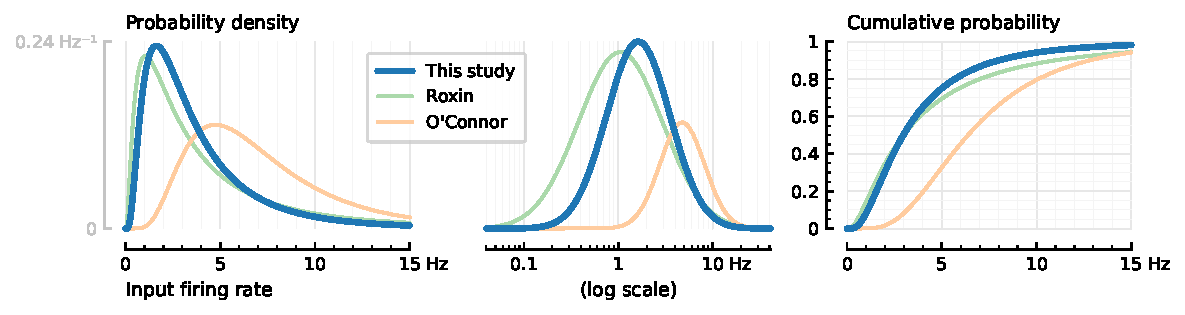
\includegraphics[w=1.6]{log-normal.pdf}
    \captionn{Input spike trains are given log-normally distributed firing rates}{The distribution used in our simulations is shown in bold. It has mean $μ_x = 4$ Hz and variance of the underlying Gaussian $\sigma^2 = 0.6$. The two light distributions are from the literature. Note that the \Citeauthor{Roxin2011DistributionFiringRates} distribution is slightly more heavy tailed than this study's: it has both more low firing and more high firing neurons.}
    \label{fig:log-normal}
\end{figure}

The firing rates of real neurons often follow a long-tailed distribution: most neurons do not fire much at all, while a few fire a lot. We recapitulate this in the firing rates of our Poisson input neurons, by drawing their firing rates from a log-normal distribution. We look to the literature for realistic parameters for this distribution, namely to the modelling paper of \Authorref{Roxin2011DistributionFiringRates}, and the experimental sources it cites \cite{Hromadka2008SparseRepresentationSounds,OConnor2010NeuralActivityBarrel}.

Log-normal distributions are usually parametrized with $μ$ and $σ$: the location and scale of the underlying normal distribution, i.e. after log-transforming the input domain. In the above sources however, the mean $μ_x$ of the data distribution itself is given. We can find $μ$, if $σ$ is known, as $μ = \ln(μ_x) - σ^2 / 2$.

\Citeauthor{Roxin2011DistributionFiringRates} use a mean rate $μ_x$ of $5$ Hz and a variance of the logarithm of the rate $σ^2 = 1.04$ in their figure 2. \Authorref{Hromadka2008SparseRepresentationSounds} recorded neurons in the auditory cortex of awake rats during acoustic stimulation. They find a mean firing rate $μ_x$ of $6.2$ Hz and a median of $2.4$ Hz; no numeric variances are given. \Authorref{OConnor2010NeuralActivityBarrel} recorded neurons in the barrel (whisker) cortex of behaving mice. Ensembled over all layers of the cortex they recorded from, they report $μ_x = 7.4$ Hz, $σ_x = 12.6$ Hz, a median of $1.5$ Hz, and an interquartile range of $9.5$ Hz. This corresponds to a Gaussian variance of $σ^2 = \ln(1 + σ_x^2 / μ_x^2) = 0.30$. The Roxin and O'Connor distributions are also shown in \cref{fig:log-normal}.

Given these data, we choose our parameters $μ$ and $σ$ so that the distribution lies roughly halfway O'Connor's and Roxin's, while making sure our firing rates are rather low than high: as our idea for connection inference rests on the number of spikes that can be used to calculate spike-triggered averages (see \cref{ch:STA}), we don't want to overestimate the number of available input spikes and obtain overly optimistic results.

Our log-normal distribution has a median of $2.96$ Hz, very close to Roxin's $2.97$ Hz. O'Connor's has $6.4$ Hz, which is markedly different from the median of $1.5$ Hz they reported (hinting that their data distribution might not be log-normal).

\subsection{Synaptic weights}

We choose to simulate EI-balanced input, where we simulate four times as many excitatory as inhibitory input spiketrains; but with the inhibitory inputs four times as strong as the excitatory inputs.

I.e. if our total number of input spiketrains is $N = 6500$, we have $N_\exc = 5200$ excitatory inputs, and $N_\inh = 1300$ inhibitory inputs. In the N-to-1-setup, we give every input of the same type the same synaptic weight. I.e. in the model summary (\cref{sec:model-summary}), $∀ i : Δg_i = Δg_\exc$ and $∀ j : Δg_j = Δg_\inh$.
If we would thus choose $Δg_\exc = 10$~pS, then, for 4:1 EI-balanced input, $Δg_\inh$ would be $40$~pS.

\marginpar{
    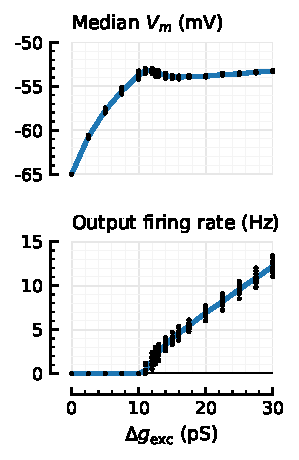
\includegraphics[w=1.04]{input_drive_we}
    \captionof{figure}{
        \textbf{Activity level of the output neuron in the N-to-1 setup, for increasing  input strength $Δg_\exc$}.\\
        \small{With $N = 6500$ EI-balanced inputs, and $Δg_\inh = 4 · Δg_\exc$.\\
        The blue line is the average over 10 different simulations (black dots), each with a different random seed for the input spike train generation.\\
        Increasing input first heightens the voltage level without increasing the firing rate, and later heightens the firing rate without increasing the voltage level further.\\
        $V_m =$ membrane voltage~$V$.\\
        Source: \nburl{2023-08-05__AdEx_Nto1_we_sweep}}.
    }
    \label{fig:input_drive_we}
}

To choose a value $Δg_\exc$ for the excitatory input strength, we look at the desired output firing rate of our one simulated neuron. We want it to spike at a realistic, average rate. Thus, we try for it to have the same output firing rate as the mean input firing rate: $μ_x = 4$~Hz. This rate is achieved by testing a range of different input drives $Δg_\exc$: see \cref{fig:input_drive_we}.
For $N = 6500$ inputs, we find an average output firing rate of $4.0$~Hz at $Δg_\exc = 15$~pS (and thus $Δg_\inh = 60$~pS).

Two asides on \cref{fig:input_drive_we}. First, from the bottom panel, we see that the AdEx model, with parameters for a cortical RS (regular spiking) neuron, is a so called `Type I' neuron:\footnote{\url{https://neuronaldynamics.epfl.ch/online/Ch4.S4.html}} the firing rate can be made arbitrarily low, and there is no discontinuous jump from 0 Hz to some minimum firing rate.

Second, why does the output activity level increase for increasing excitatory input, if the inhibitory input becomes stronger by the same amount? The answer lies in the synaptic reversal potentials, which are $E_\exc = -80$~mV and $E_\inh = 0$~mV. The median membrane voltage (top panel in \cref{fig:input_drive_we}), at about $-60$~mV, lies closer to the inhibitory reversal potential than the excitatory potential, making the inhibitory term of the synaptic current $I_\syn$ weaker than the excitatory term  (\cref{eq:I_syn_simple}).

\begin{figure}
    \begin{sidecaption}
        {\textbf{The different signals in the conductance-based AdEx model}.\\
        \small{Example signal traces. N-to-1 setup, with $N = 6500$ EI-balanced input spiketrains, and $Δg_\exc = 15$~pS. Neuron parameters for a cortical regular spiking neuron.\\
        Note that the synaptic current signal $-I_\syn$ is very similar to the difference of the excitatory and inhibitory synaptic conductances, as long as the membrane voltage $V$ does not vary too much; on a spike (here at $t ≈ 680$~ms), $I_\syn$ spikes as well.\\
        Also note that the neuron spikes at a time when the inhibitory input randomly falls below the excitatory input, for a certain time. Spikes are 'fluctuation driven' in this input regime.\\
        $g_e ≡ g_\exc$ and $g_i ≡ g_\inh$.\\
        The $V$ and $-I_\syn$ signals are cut-off by the plot boundaries at the spike time. \\
        Source: \nburl{2023-07-26__AdEx_Nto1_we_I_syn}.}
        }
        [fig:all_sigs_6500]
        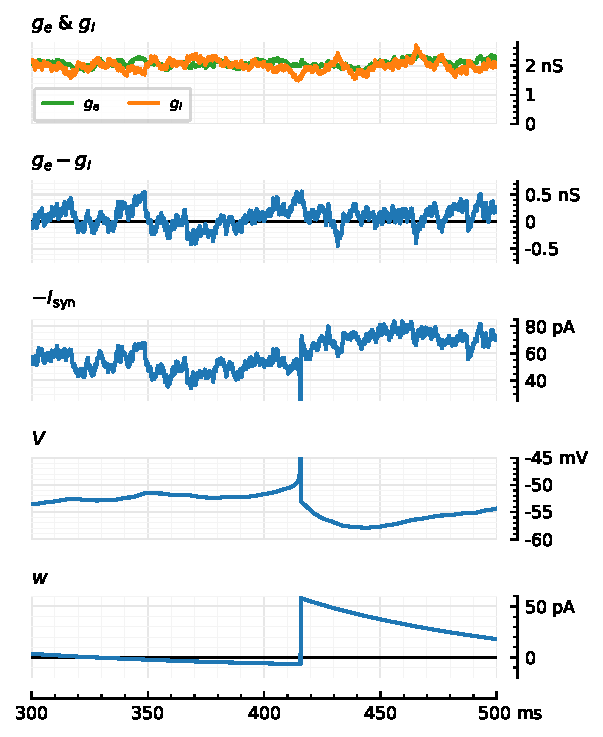
\includegraphics[w=1.04]{all_sigs_6500}
    \end{sidecaption}
\end{figure}

The fact that this EI-balanced input leads to a net-excitatory effect can also be seen in \cref{fig:all_sigs_6500}: the signal $g_\exc - g_\inh$ hovers around zero, but the signal $I_\syn$ ---~even though it has largely the same shape~--- is nowhere near zero.


Later, we will compare the performance of a connection-detection algorithm across different numbers of inputs $N$. We choose the approximately evenly log-spaced sequence
\begin{equation*}
    N ∈ [10,\ 20,\ 45,\ 100,\ 200,\ 400,\ 800,\ 1600,\ 3200,\ 6500].
\end{equation*}
For each of these $N$, we want the output firing rate to be the same, namely 4~Hz. To find the synaptic strengths $Δg_\exc$ that accomplish this, we perform an iterative search.\footnote{We use SciPy's \texttt{root\_scalar} function, which uses `Brent's method', which is like bisection but has faster convergence. We seed the algorithm with the bracket $[w_0/4, w_0·4]$, where $w_0$ is the initial linear guess for $Δg_\exc$. In about 8 iterations, we come within $0.01$~Hz of the desired $4$~Hz.}
As an initial guess, it would make sense for the required input strength to scale inversely proportional to the number of inputs. We find however that there is a slight deviation from this linear expectation (\cref{fig:we-for-4Hz-for-all-N}): the less inputs, the less strong each input should be to reach the same output firing rate, compared to a linear extrapolation from our finding of $Δg_\exc = 15$~pS for $N = 6500$.
E.g. the linear expectation for $N = 10$ would be $Δg_\exc = 9.75$~nS ($= 15 \text{ pS} · 6500 / 10$), but we find we need only $Δg_\exc = 2.83$~nS to reach an output firing rate of $4$~Hz.

\begin{figure}
    \begin{sidecaption}
        {\textbf{Finding the right input strength in the N-to-1 setup, for different numbers of inputs $N$}.\\
        \small{For each $N$, the right input strength $Δg_\exc$ (namely the one for which the output neuron fires at $4$~Hz) was found using an iterative search procedure. For every $Δg_\exc$ value evaluated, ten different 10-second simulations were run (each with a different random seed for the input spiketrain generation). The average output firing rate of these ten simulations was taken, and compared with the goal firing rate of $4$~Hz. $Δg_\exc$ was then adjusted until the simulated firing rate was sufficiently close.\\
        Source: \nburl{2023-08-05__AdEx_Nto1_we_sweep}.}
        }
        [fig:we-for-4Hz-for-all-N]
        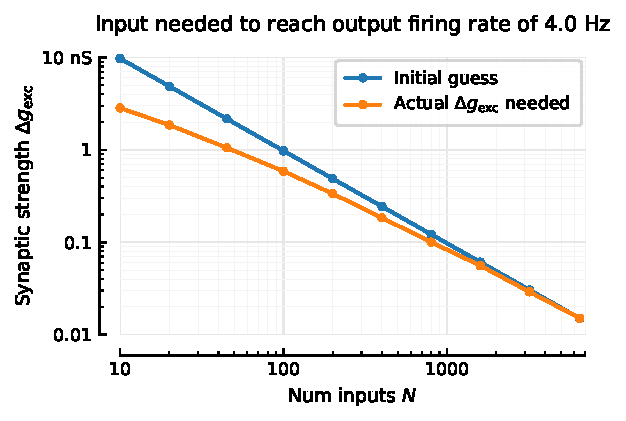
\includegraphics[w=0.85]{we-for-4Hz-for-all-N}
    \end{sidecaption}
\end{figure}


\FloatBarrier
\section{Voltage imaging}

The signals detected by a light microscope in a voltage imaging setup are not the same as the real membrane voltage traces of which they are a reflection.

We model this lossy transformation by simply adding Gaussian noise to our simulated membrane voltage. As in the voltage imaging literature, we quantify the amount of this  noise by a `spike-SNR' measure (spike signal-to-noise ratio). This is defined as the height of an average spike relative to the standard deviation of the noise:
\begin{equation}
    \text{spike-SNR} = \frac{\text{spike height}}{σ_\text{noise}}
\end{equation}

\marginpar{
    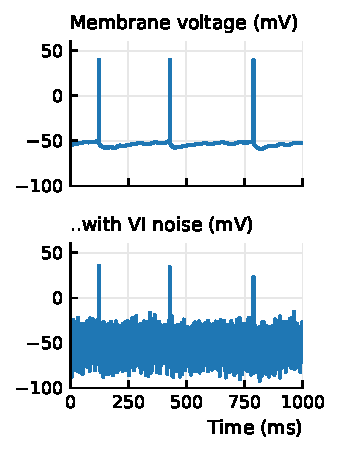
\includegraphics[w=1]{VI_noise.pdf}
    \captionof{figure}{Simulated voltage trace (same as in \cref{fig:Vm_Izh_vs_AdEx}, right), without and with `voltage imaging' (VI) noise added ($σ_\text{noise} = 10.5$~mV).}
    \label{fig:VI_noise}
}

In other words, if we call our output signal $y$, and with $V_i$ the voltage samples resulting from the numeric integration of \cref{eq:AdEx-V}, we have:
\begin{gather}
    y_i = V_i + ε_i \\[1em]
    ε_i \sim \mathcal{N}(0, σ_\text{noise}) \notag
\end{gather}

A typical but conservative level of noise in voltage imaging recordings has a spike-SNR of $10$. If we take as spike height the spike detection threshold minus the leak potential ($θ - E_L$, see \cref{tab:AdEx-params}), we obtain a $σ_\text{noise}$ of $10.5$~mV.

A more realistic model of the voltage imaging-transformation would also incorporate the exponential decay over time of the SNR (with a time constant of about 10 minutes), and the short-term 'smearing in time' of voltage indicators. The latter could be done by passing the voltage signal through a linear filter with some non-instantaneous impulse response.



\section{Software implementation}
\label{sec:software}

To numerically simulate the model described in this chapter, different software implementations have been used throughout my PhD.

\begin{table}[h]
    \begin{sidecaption}
        {\textbf{Time taken to simulate 10 seconds of the N-to-1 experiment}
        {\small with N = 6500 Poisson inputs, and one conductance-based AdEx neuron. In the `merged' models, only 200 Poisson spiketrains are independently simulated (instead of all 6500, as in the `full' model). All other inputs are replaced by two single Poisson inputs (one excitatory and one inhibitory), with an equivalent effect. (That is, we use Brian's `\texttt{\href{https://brian2.readthedocs.io/en/stable/user/input.html\#efficient-poisson-inputs-via-poissoninput}{PoissonInput}}').\\
        For details, see \nburl{2023-07-10__AdEx_Nto1_Brian_speedtest} (Cython), \nburl{2023-08-02__speedtest_brian_standalone_AdEx_Nto1} (C++), and \nburl{2023_08_09__Poisson_cquantile_upperbound} (Julia).}
        }
        [tab:software-timings]
            \begin{tabular}{l l l S[table-format=2.2] S[table-format=2.3]}
            % last two cols are an siunitx thing to align on decimal point.
            \toprule
            Software & Language & Model  &  \multicolumn{2}{l}{Time (seconds)} \\
                     &   &   &  {Compilation} & {Simulation}\\
            \addlinespace[0.3em]
            \midrule
            \addlinespace[0.7em]
            Brian2 &  Cython + Python   & full  & 61  &   11  \\
                        &                              & merged  & 86  &  11  \\[0.7em]
                         &  C++                    & full           & 15  &  6.5  \\
                        &                             & merged  & 18  &  0.35  \\[0.7em]
            own &  Julia                     & full       &  0.68  &  0.036  \\
            \bottomrule
        \end{tabular}
    \end{sidecaption}
\end{table}

% Note that the timings in \cref{tab:software-timings} do not include compilation times, which can be considerable.

\emph{\{to expand a bit\}}
